\chapter{\mc 従来手法を用いた足動作検知のための\rm BCI}
従来手法の枠組みによって構築した足動作検知のBCIについて説明する。
\section{\mc 計測した\rm EEG\mc について}
まず、被験者が8秒間静止(以後rest状態)と
8秒間足動作(以後walk状態)を8サイクル繰り返したときのEEGを計測した。
被験者はリラックスできる椅子に着席した状態で前方に配置されたディスプレイの
指示に従って動作を行った(図\ref{fig:asibumi})。
ただし、8サイクル中最初の1サイクルについてはフィルタの応答の特性上、
EEGの解析には適さないと判断し、解析時には除外した。
従って以後の解析で用いられるのは7サイクル分のEEGである。
EEGの計測機器としてはg.tec社のg.USBamp(図\ref{fig:usbamp})を用い、ウェット式の電極を採用した。
ウェット式では頭皮と電極の間に導電性のジェルを注入することでEEGを計測する。
EEGの計測時にはジェルの注入を行いながら、すべての電極に関して電極インピーダンスが\(5k\Omega\)
以下になったことを確認した。
またサンプリング周波数は128Hzとした。
\begin{figure}
    \centering
    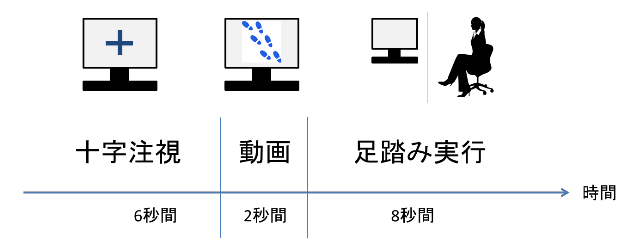
\includegraphics[width=13cm]{images/asibumi.png}
    \caption{EEG計測時のタイムスケジュール}
    \label{fig:asibumi}
\end{figure}
\begin{figure}
    \centering
    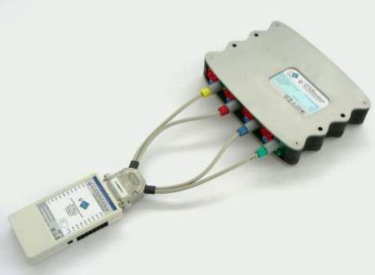
\includegraphics[width=8cm]{images/usbamp.png}
    \caption{g.tec社のg.USBamp}
    \label{fig:usbamp}
\end{figure}

計測に用いた電極の個数は5つであり、Cz、C1、C2、CPz、FCz電極である。
Cz電極は足に関する運動野が脳の頭頂部に存在するため選出し、
スモールラプラシアンフィルタが適用できるように残りの4つを選出した(図\ref{fig:smalllap})。
また、EEGの計測時には定常成分とERDとは無関係な高周波成分を削除するために
通過帯域を0.3Hzから36Hzとした2次のバタワースバンドパスフィルタを用いた。

\section{\rm EEG \mc の解析}
\subsection{\mc スペクトル密度推定による\rm ERD\mc の確認}
まずCz電極で計測されたEEGと
Cz電極に対してスモールラプラシアンフィルタを用いた際の
EEGを図\ref{fig:eegsub1}に添付する。
ここで、\(x_{A}(t)\)はA電極によって計測された波形であるとして
Cz電極に対してスモールラプラシアンフィルタを用いた際の波形\(z(t)\)は以下である。
\begin{equation}
    z(t) = x_{Cz}(t) - \frac{1}{4}(x_{C1}(t) + x_{C2}(t) + x_{FCz}(t) + x_{CPz}(t))
\end{equation}
スモールラプラシアンフィルタの定義から、
頭皮上でCz電極に際立った電位分布が獲得されていることが期待できる。

\begin{figure}
    \centering
    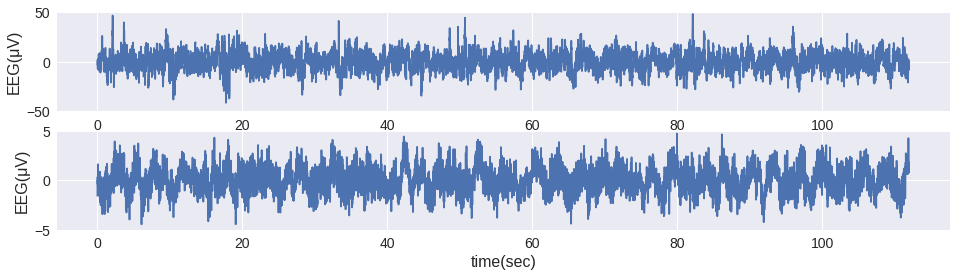
\includegraphics[width=13cm]{images/eeg_sub1.png}
    \caption{Cz電極のEEG(上)とスモールラプラシアンフィルタを用いたEEG(下)}
    \label{fig:eegsub1}
\end{figure}
% \begin{figure}
%     \centering
%     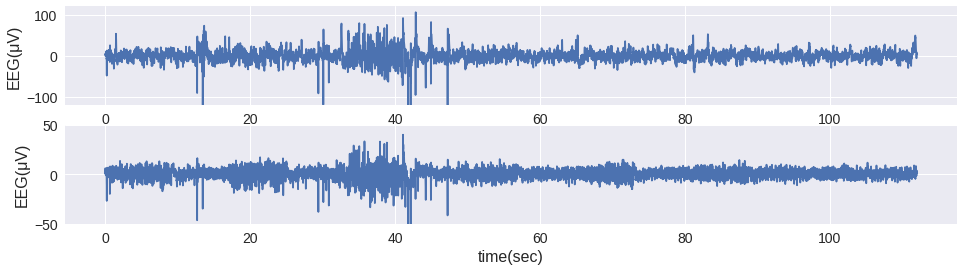
\includegraphics[width=13cm]{images/eeg_sub2.png}
%     \caption{被験者2のCz電極のEEG(上)とスモールラプラシアンフィルタを用いたEEG(下)}
%     \label{fig:eegsub2}
% \end{figure}

% 続いて、PCAとICAによる空間フィルタの設計を試みた。
% それぞれのフィルタから得られる各被験者のEEGの波形を図\ref{fig:bss1}と図\ref{fig:bss2}に示す。
% が\label{section:BSS}にて述べた問題のために、
% 得られた信号のいずれが重要であるかの判断を行うことができなかった。

次にスモールラプラシアンフィルタを用いたEEGの
rest状態(8秒間)の波形とwalk状態(8秒間)の波形それぞれに対してパワースペクトル密度推定を行った。
スペクトル密度推定には1秒間(128点)の時間窓を用いたウェルチのオーバラップ法を利用し、
オーバラップは0.5秒(64点)とした。
rest状態とwalk状態は計7回繰り返し行なっているため図\ref{fig:allERDs}に
7回分すべてのスペクトル密度の比較を示す。
また図\ref{fig:walkERD}に7回分の平均を示す。
ERDの生ずる周波数帯域は個人差があるとされるが、
\(\mu\)律動(8-12Hz)や\(\beta\)律動(18-26Hz)で
パワーの減少が観測できる報告があり\cite{erdfreq}、また\cite{Beta波によるBCI}では
6-40Hzの領域に渡ってERDを検知しBCIを構築した例がある。
概ね先行研究において観測されている周波数帯域でwalk時のパワーの減少が確認された。
\begin{figure}
    \centering
    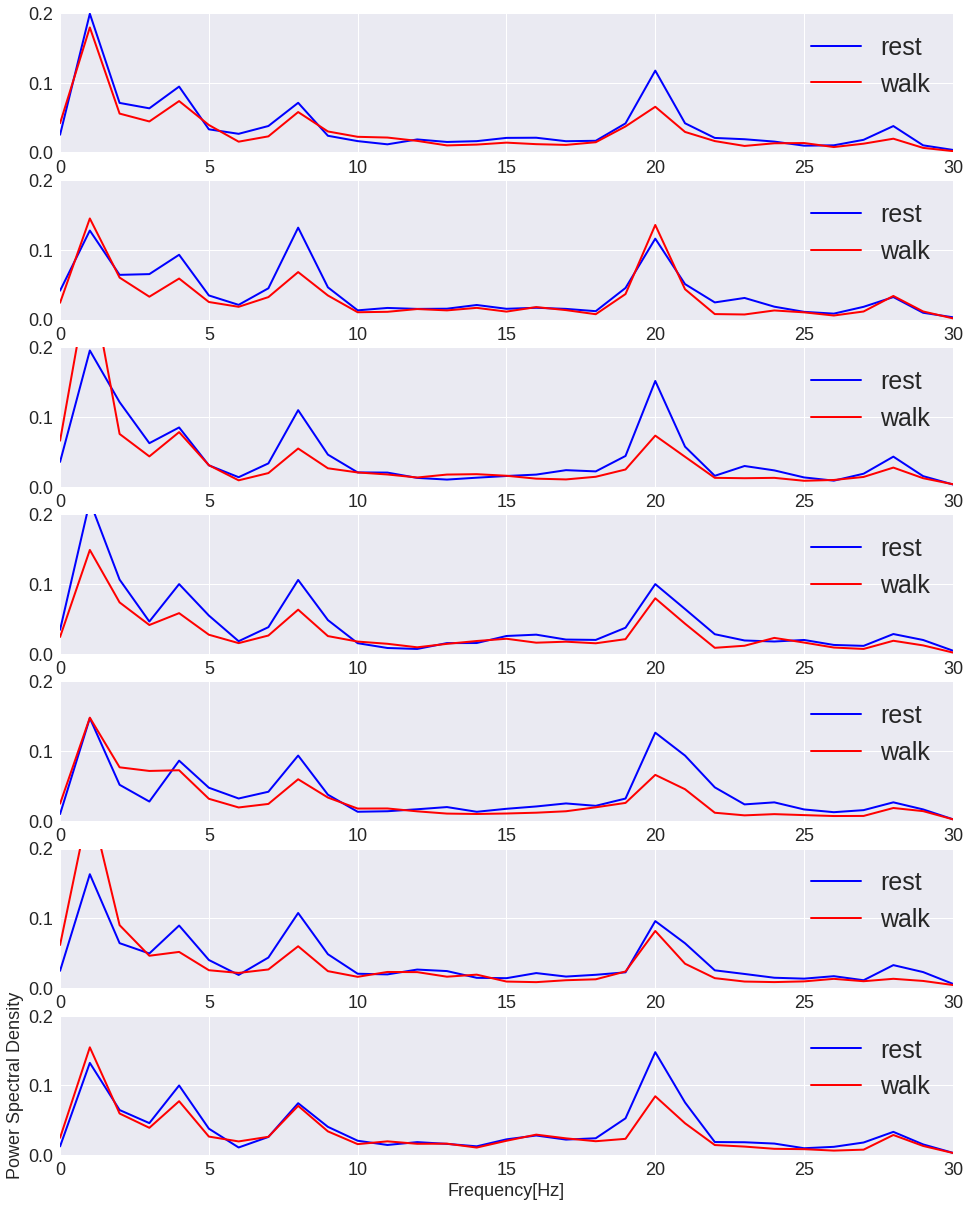
\includegraphics[width=13cm]{images/allERDs}
    \caption{rest時とwalk時のパワースペクトル密度の比較}
    \label{fig:allERDs}
\end{figure}
\begin{figure}
    \centering
    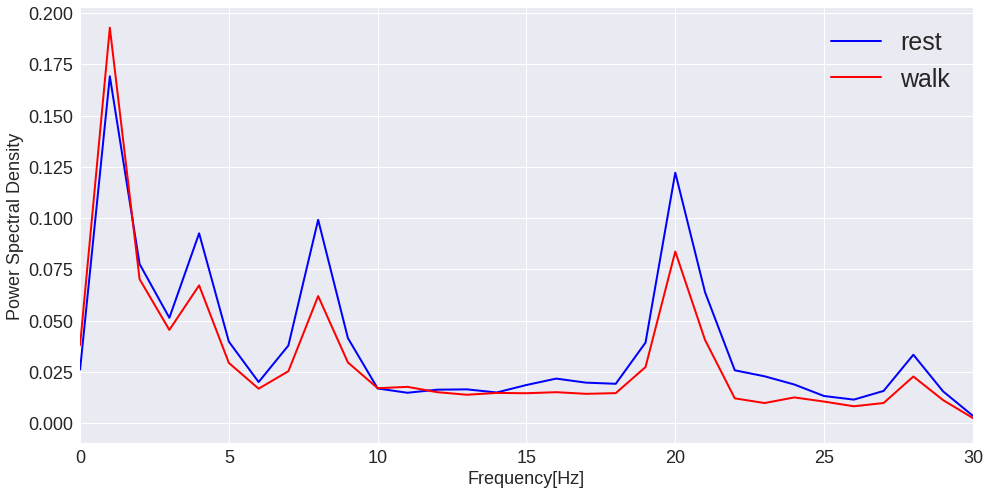
\includegraphics[width=13cm]{images/walkERD}
    \caption{rest時とwalk時のパワースペクトル密度の平均(7回分)の比較}
    \label{fig:walkERD}
\end{figure}

しかし、平均(図\ref{fig:walkERD})を確認すると
4、8、20Hz付近で際立ったパワーの減少が見られるが、
個々のスペクトル密度(図\ref{fig:allERDs})は必ずしもパワーの減少が
すべてのサイクルで同様に確認できることを示してはいない。
例として20Hzで際立ったパワーの減少(ERD)が生ずると考えた場合には、
図\ref{fig:allERDs}の上から2番目に関しては検知ができないことになる。
従って、ERDを検知してBCIを動作させることを考える場合には、
複数の周波数帯域のパワーを総合的に評価する必要があると考えられる。

また、パワースペクトル密度の絶対値を評価するよりも
rest状態とwalk状態の相対的なパワーの差の方が重要であることが言える。
例として、図\ref{fig:walkERD}から20Hzのパワースペクトル密度が0.1以下になった場合に
walk状態であると判定するBCIは図\ref{fig:allERDs}の下から二番目のグラフの
rest状態をwalk状態と判定することになる。
パワーの絶対値がさほど重要な指標にならないことは、
EEGの計測が電極のインピーダンス(ジェルの塗布状況)や
頭皮のインピーダンス(皮脂や毛髪)に左右されることからも想定されることである。

従ってERDを検知するためには複数の周波数帯域に跨って、
rest状態とwalk状態の相対的なパワーの変化に着目する必要があると考えた。


\subsection{\mc 足動作検知のための信号処理}
解析結果に基づいて、EEGに対して以下の信号処理によって特徴量を獲得した。
\begin{enumerate}
    \item 2種類のバンドパスフィルタ:通過帯域を3-14Hzと13-33Hz
    \item スモールラプラシアンフィルタ:Cz電極に適用
    \item バーグ法によるスペクトル密度推定:時間窓を1秒(128点)、オーバラップ127点
    \item ローパスフィルタ:スペクトル密度の時間変化の平滑化
    \item ハイパスフィルタ:パワースペクトル密度の時間変化の定常成分カット
\end{enumerate}
上記の処理における1.〜5.の概略図を図\ref{fig:footBCI}に示す。
\begin{figure}
    \centering
    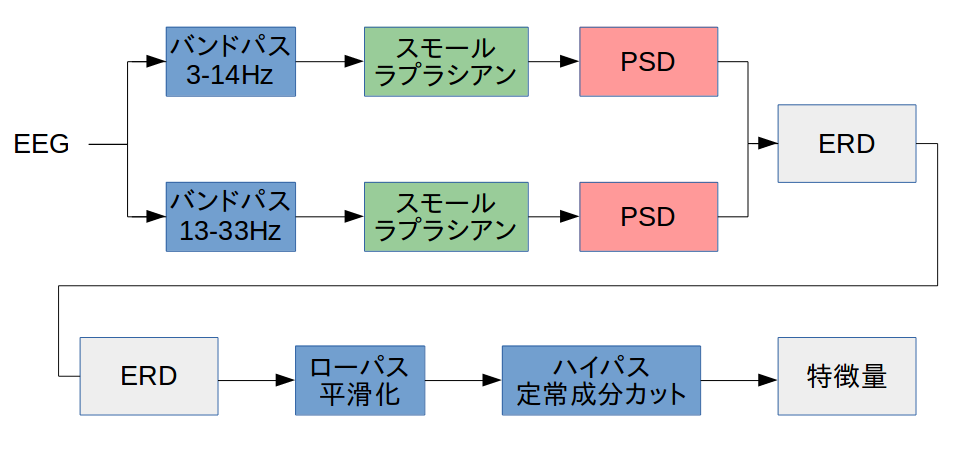
\includegraphics[width=13cm]{images/prepro.png}
    \caption{EEGから特徴量を獲得する処理の流れ}
    \label{fig:footBCI}
\end{figure}
1.〜3.の処理では2種類のバンドパスフィルタを通過したEEGに対してそれぞれスペクトル密度推定が行われる。
3−14Hzのバンドパスフィルタを通過した波形に関しては、パワースペクトル密度の4-13Hzのみを利用し、
13−33Hzのバンドパスフィルタを通過した波形に関しては、パワースペクトル密度の15-32Hzのみを利用した。
この着目する帯域は、EEGの\(\alpha\)律動及び\(\mu\)律動、\(\beta\)律動などの周波数帯域と
解析したEEGのピークの位置を加味し、経験的に定めた。
時間窓は1秒間であるため周波数分解能は1Hzであり、各時間窓において計28の特徴量が得られる。
時間窓は1サンプル点ずつ移動させるため、1/128秒毎に28次元の特徴量が出力される。
図\ref{fig:nofilterERD}に1.〜3.の処理を施した出力を添付する。
\begin{figure}[p]
    \centering
    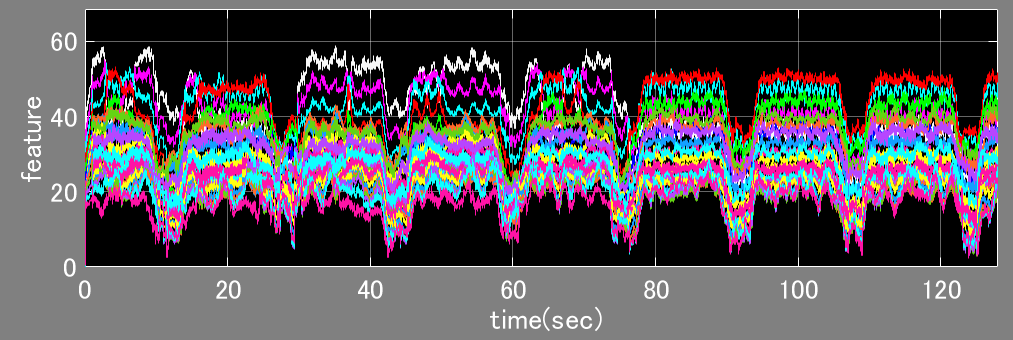
\includegraphics[width=13cm]{images/feature_sub1_nofilter.png}
    \caption{28個の特徴量の時間変化}
    \label{fig:nofilterERD}
\end{figure}
図\ref{fig:nofilterERD}からは、
特徴量が全体的に減少している様子が8回分観測できる。
また特徴量はパワースペクトル密度の時間変化に他ならないため、
特徴量の減少はERDであり8回の足動作に由来していると考えられる。

次に、特徴量の変化がrest状態とwalk状態において際立つことが重要であり、
同一状態においては変化が少ない方が好ましいことを考慮し
4.ローパスフィルタによる平滑化を行った。この処理によって、
状態が切り替わる程の大きな特徴量の変化が強調される(図\ref{fig:lfilterERD})。
\begin{figure}[p]
    \centering
    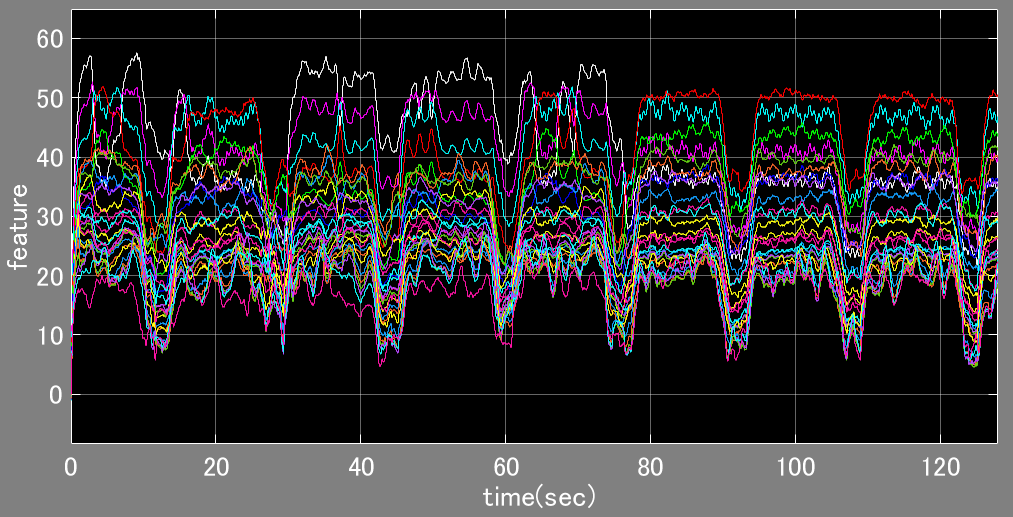
\includegraphics[width=13cm]{images/feature_sub1_l.png}
    \caption{ローパスフィルタを追加した28個の特徴量の時間変化}
    \label{fig:lfilterERD}
\end{figure}

また、ERDを検知する場合には
rest状態とwalk状態の各状態間のパワースペクトル密度の相対的差異が重要である
と考えられることを前述した。
同時に、分類器にとっても相対的差異のみが重要であり絶対値は影響しないことを考慮し、
5.ハイパスフィルタによって定常成分をカットした(図\ref{fig:filterERD})。
\begin{figure}[p]
    \centering
    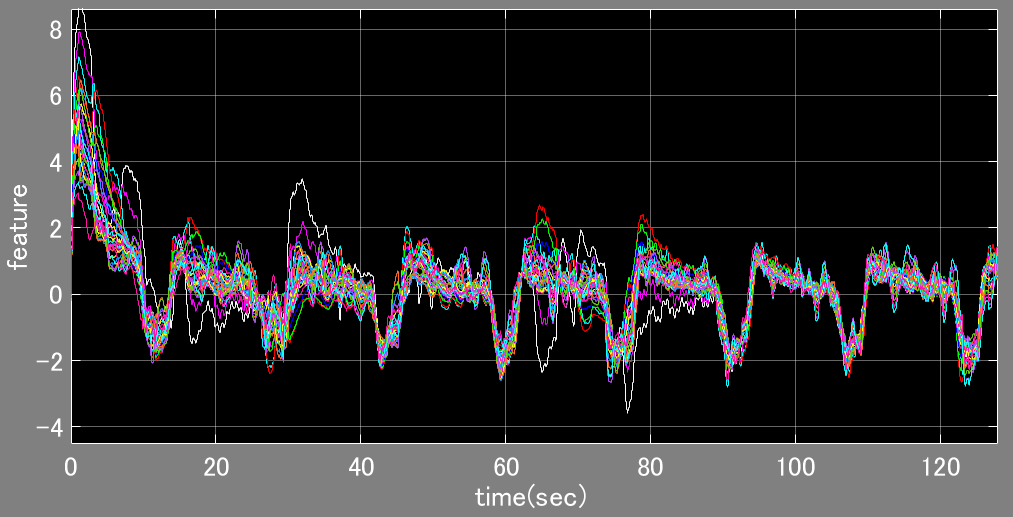
\includegraphics[width=13cm]{images/feature_sub1.png}
    \caption{ローパスフィルタとハイパスフィルタを追加した28個の特徴量の時間変化}
    \label{fig:filterERD}
\end{figure}

バーグ法によるスペクトル密度推定値をピリオドグラムに置き換え、
同様の処理を行った際の特徴量の時間変化を図\ref{fig:fftERD}に示す。
またバーグ法をウェルチのピリオドグラム法で置き換えた際の特徴量の時間変化を
図\ref{fig:welchERD}に示す。
いずれもスペクトル密度推定として広く用いられる方法であるが、バーグ法を用いた
場合のスペクトル密度の時間変化(図\ref{fig:filterERD})は
特徴量(ERD)が目視できるほどに強調されていることが分かる。

\begin{figure}[tp]
    \centering
    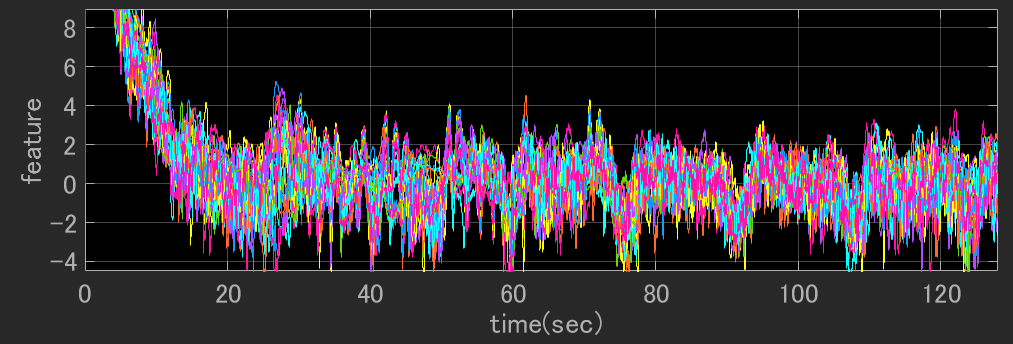
\includegraphics[width=13cm]{images/feature_sub1_fft.png}
    \caption{ピリオドグラムを用いた28個の特徴量の時間変化}
    \label{fig:fftERD}
\end{figure}
\begin{figure}[tp]
    \centering
    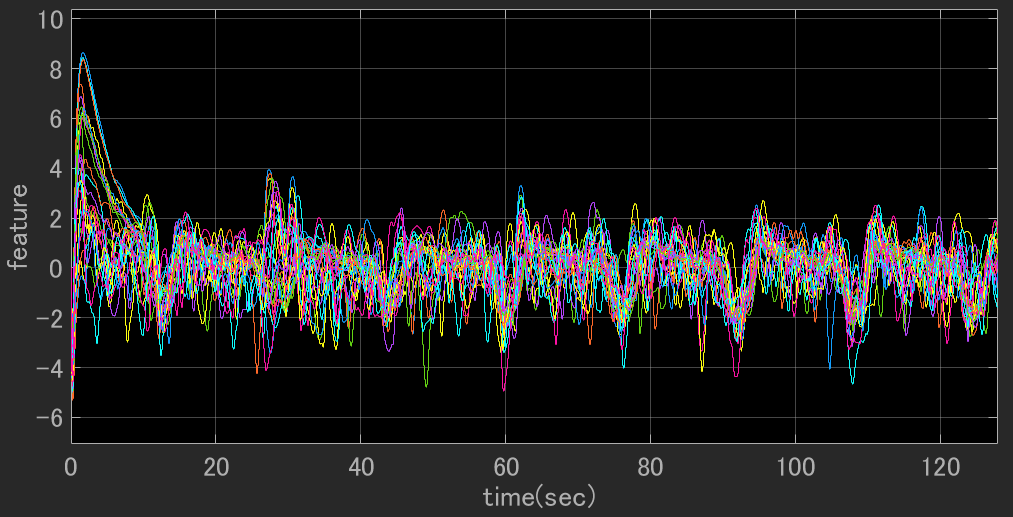
\includegraphics[width=13cm]{images/feature_sub1_welch.png}
    \caption{ウェルチのピリオドグラム法を用いた28個の特徴量の時間変化}
    \label{fig:welchERD}
\end{figure}

\subsection{\mc 次元削減と分類}
ここまでの処理によって得られた特徴量の次元は28であり、以後\(x_i \in \mathbb R^{28}\)と表記する。
ここに\(i\)はサンプル時刻を表すインデックスである。
\(x_i\)はサンプル時刻\(i\)における特徴量を格納しており、
特徴量はERDを強調するための処理が施されたものである。
仮に特徴量\(x_i\)を引数としてrest状態かwalk状態を識別する分類器\(y_i=f(x_i)\)を、
\ref{section:discriminant}で述べた手法によって構築することを考えた場合には、
時刻の情報を完全に破棄して各時刻の\(x_i\)に対して個々に分類を行うことになる。
フィルタの特性上EEG計測時の最初のサイクルは学習データとして用いないこととし、
データ点数は14336点(\(i=1,\cdots,14336\))となる。各点の正解ラベルは
EEG計測時のrest状態を\(0\)、walk状態を\(1\)とした(図\ref{fig:targetsignal})。
この条件の下で7交差検証によりAccuracyを算出した結果、
ロジスティック回帰では82.6\%となった。
また同一被験者の新規EEGから抽出した特徴量(14336点)に対してのテストAccuracyは72.9\%となった。

交差検証により得られたAccuracyに比べ、新規のデータに対するAccuracyが低くなっている。
交差検証は分類器の汎化性能を評価する一般的な方法であるが、
EEGの場合は同一被験者であったとしても頭皮やジェルの状況に応じて波形の性質が異なる場合がある。
そこで28次元の特徴量をPCAにより次元削減することで、
有用な情報を1つの成分に集約する。
PCAでは変換先で各成分が無相関となるため、
言い換えると変換前において相関のある成分は適切な線型結合によって1つの成分に集約される。
今回の場合はERDを抽出することから開始したために、
28次元の特徴量の各成分は明らかに相関性を有しており(図\ref{fig:filterERD})、
PCAが適していると判断した。
更にERDとは関係のない成分を除外する役割を担うことも期待できる。

PCAを次元削減に用いた場合、ロジスティック回帰の交差検証Accuracyは78.7\%となった。
一方でテストAccurcyは84.2\%となった。
続いて、他の被験者に対しても同様にEEGを計測し分類器を構築した。
PCAを用いない場合の交差検証Accuracyは88.3\%となり、テストAccuracyは69.6\%となった。
PCAを用いた場合の交差検証Accuracyは85.5\%となり、テストAccuracyは72.9\%となった。

そこで、\(x_i\)を28個並べたベクトル\(z_i=(x_i^T, x_{i+1}^T,\cdots, x_{i+27}^T)^T\ \in \mathbb R^{784}\)
を導入する。分類器\(y_i=f(z_i)\)を考えた場合には各時刻の\(z_i\)に対して個々に分類を行うことになるが、
\(z_i\)は28点分の時刻の情報を有しているため、分類器は\(x_i\)の時間変化を取り入れた学習が可能である。

線形判別分析77.8\%
ロジスティック回帰82.6\%

線形判別分析78.1\%
ロジスティック回帰82.6\%